\section{Dil İşlemcileri}

Basitçe, derleyici, bir dilde yazılmış -\textit{kaynak} dil- herhangi bir programı okuyup başka bir dile -\textit{hedef} dil -  eşdeğer olarak çeviren bir programdır; bkz. Şekil 1.1. Derleyicinin önemli bir rölü, dönüşüm sırasında kaynak dilde tespit ettiği hataları bildirmesidir.

\begin{center}
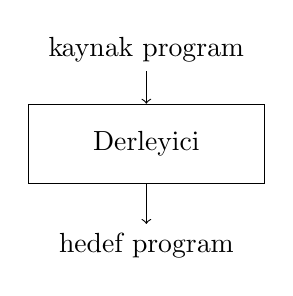
\begin{tikzpicture}[->]

\tikzstyle{rect} = [rectangle, minimum width=3cm, minimum height=1cm,text centered, draw=black]
\node (src)  {kaynak program};
\node (tr) [below of=src, yshift=-1.5cm] {hedef program};
\node (dr) [rect, below of=src, yshift=-0.2cm] {Derleyici};   
   
\draw [black](src) -- (dr);  
\draw [black](dr) -- (tr);  

\end{tikzpicture}

Şekil 1.1: Bir derleyici
\end{center}



Eğer hedef program çalıştırılabilir bir makine-dili programıysa, kullanıcı tarafından girdileri işlemesi ve çıktı üretmesi için kullanılabilir; bkz. Şekil 1.2.

\begin{center}
\begin{tikzpicture}[->]

\tikzstyle{rect} = [rectangle, minimum width=3cm, minimum height=1.5cm,text centered, draw=black]

\node (in) [left of=src, xshift=-1.5cm] {girdi};
\node (out)[right of=src, xshift=1.5cm]   {çıktı};
\node (tr) [rect] {Hedef Program};   
   
\draw [black](in) -- (tr);  
\draw [black](tr) -- (out);  

\end{tikzpicture}

Şekil 1.2: Hedef Programı Çalıştırmak

\end{center}

\renewcommand{\thefootnote}{\fnsymbol{footnote}}
\textit{Yorumlayıcı\footnote{(İng.) Interpreter. (Ç.N.)}} da yaygın bir dil işlemci tipidir. Şekil 1.3'te görüldüğü gibi hedef programını üretirken bunu çevrim olarak yapmaktansa, yorumlayıcı, kaynak programın içindeki komutları direkt olarak, kullanıcı tarafından sağlanan girdiler üzerinden çalıştırır.

\begin{center}
\begin{tikzpicture}[->]

\tikzstyle{rect} = [rectangle, minimum width=3cm, minimum height=1.5cm,text centered, draw=black]

\node (in) [left of=src, xshift=-1.5cm, yshift=-0.3cm] {girdi};
\node (src) [left of=src, xshift=-3cm, yshift=0.4cm] {kaynak program};
\node (out)[right of=src, xshift=6cm,yshift=-0.4cm]   {çıktı};
\node (tr) [rect] {Yorumlayıcı};   
   
\draw [black](in) -- (tr.192);  
\draw [black](src) -- (tr.165);  
\draw [black](tr) -- (out);  

\end{tikzpicture}

Şekil 1.3: Hedef Programı Çalıştırmak
\end{center}


Girdileri çıktılara eşleyen bir yorumlayıcıdansa, derleyici tarafından üretilmiş bir makine-dili hedef programı genellikle daha hızlıdır. Bununla beraber, bir yorumlayıcı, hataları genellikle bir derleyiciden daha iyi teşhis edebilir, çünkü yorumlayıcı kaynak programı satır satır çalıştırır.

\paragraph{Örnek 1.1:}
Şekil 1.4'te görüldüğü gibi Java dil işlemcileri derlemeyi ve yorumlamayı beraber kullanır. Java kaynak programı önce \textit{bytecode} denilen bir ara form'a çevrilir. Ardından bytecode'lar bir sanal makine tarafından yorumlanır. Bu tür bir ayarlamanın avantajı, bir makinede derlenen bir kodun başka bir makinede ya da bir ağ üzerindeki makinelerde yorumlanabilmesidir.

Girdilerin çıktılara dönüştürülmesini hızlandırmak için, \textit{tam-zamanında} derleyiciler denilen bazı Java derleyicileri, bytecode'ları ara program girdileri işlemeden önce,  anlık olarak makine diline çevirir. 

\begin{center}
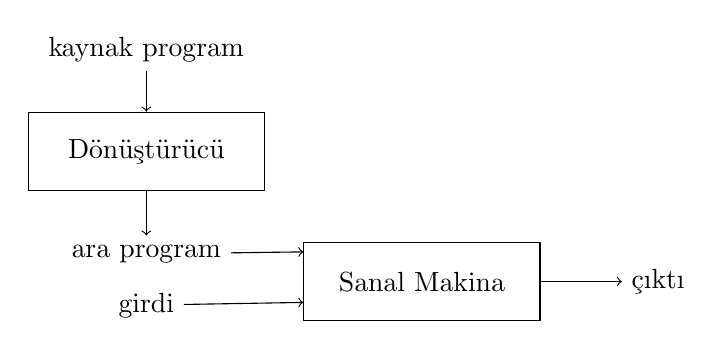
\begin{tikzpicture}[->]

\tikzstyle{rect} = [rectangle, minimum width=3cm, minimum height=1cm,text centered, draw=black]

\node (src_p)   {kaynak program};
\node (translator) [rect, below of=src_p, yshift=-0.3cm] {Dönüştürücü};   
\node (intermediate_p) [below of=translator, yshift=-0.3cm] {ara program};
\node (in) [below of=intermediate_p, yshift=0.35cm] {girdi};
\node (vm) [rect, right of=in, xshift=2.5cm, yshift=0.3cm, ] {Sanal Makina};   
\node (out) [right of=vm,xshift=2cm] {çıktı};

\draw [black](src_p) -- (translator);  
\draw [black](translator) -- (intermediate_p);  
\draw [black](intermediate_p) -- (vm.166);  
\draw [black](in) -- (vm.190);  
\draw [black](vm) -- (out);  

\end{tikzpicture}

Şekil 1.4: Bir hibrid derleyici
\end{center}

Şekil 1.5'te gösterildiği gibi bir derleyiciye ek olarak, çalıştırılabilir bir hedef program oluşturmak için birkaç program daha gerekli olabilir. Bir kaynak program ayrı dosyalarda tutulan modüllerden oluşmuş olabilir. Bu kaynak kodu toparlamak bazen \textit{önişlemci} denlilen başka programlara havale edilir. Önişlemci ayrıca makro denilen kısayolları kaynak kodun ifadelerine çevirebilir.

Ardından düzenlenmiş kaynak kodu derleyiciye yüklenir. Derleyici çıktısı olarak assembly-dili programı üretebilir, çünkü assembly üretimi ve hata ayıklaması kolay bir programdır. Ardından assembly dili, yeniden konumlandırılabilir makine kodu üreten ve \textit{assembler} denilen bir programda işlenir.

Büyük programlar genelde parçalar halinde derlenir, böylece yeniden konumlandırılabilir makina kodu, makinada çalışan diğer yeniden konumlandırılabilir nesne ve kütüphane dosyaları ile bağlanabilir. \textit{Bağlayıcı} bir dosyadaki dosyanın başka bi dosyadaki dosyaya ulaşması için harici hafıza adreslerini çözümler. \textit{Yükleyici} sonra tüm bu çalıştırılabilir nesne dosyalarını bir araya getirip çalıştırılmak üzere hafızaya yükler.  

\subsection{Bölüm 1.1 için Alıştırmalar}

\paragraph{Örnek 1.1.1:} Bir yorumlayıcı ile derleyicinin arasındaki fark nedir?

\paragraph{Örnek 1.1.2:}  a ve b maddelerin avantajları nelerdir?; a) Bir yorumlayıcı üzerine bir derleyici. b) Bir derleyici üzerine bir yorumlayıcı.

\paragraph{Örnek 1.1.3:} Derleyicinin makina dilindense assembly dili ürettiği bir dil-işleme sisteminin avantajları nelerdir?

\paragraph{Örnek 1.1.4:} Yüksek seviyeli bir dili başka yüksek seviyeli bir dile çeviren derleyiciye \textit{kaynaktan-kaynağa} dönüştürücü denir. C dilini bir derleyici için kaynak dil olarak kullanmanın avantajları ne olur?

\setcounter{footnote}{0}
\paragraph{Örnek 1.1.5:}  Bir çevirici'nin\footnote{(İng.) Assembler. (Ç.N.)} görevlerinden birkaçını tanımlayın.

\begin{center}
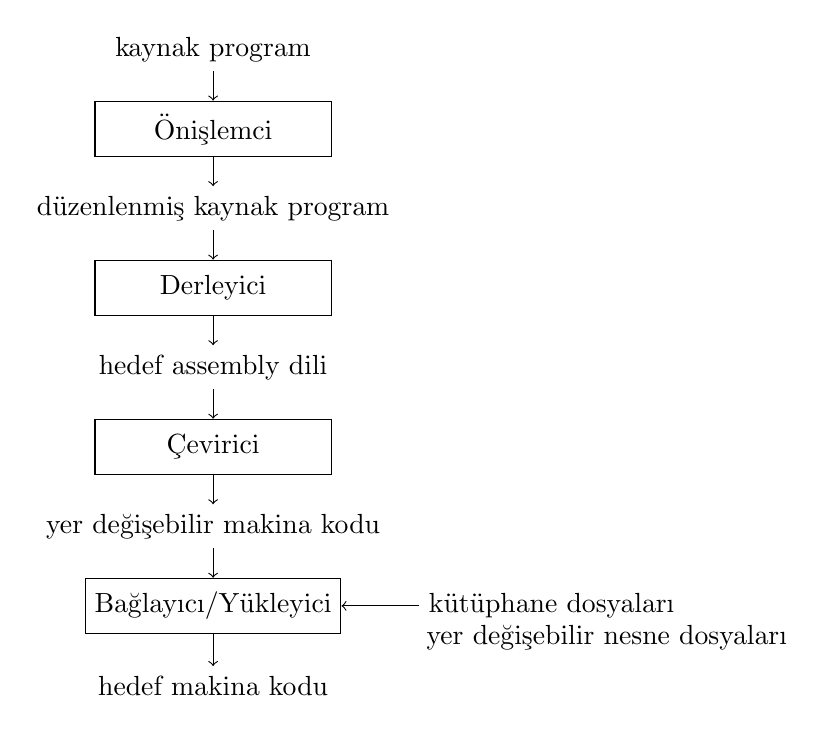
\begin{tikzpicture}[->]

\tikzstyle{rect} = [rectangle, minimum width=3cm, minimum height=0.7cm,text centered, draw=black]

\node (src_p)   {kaynak program};
\node (prep) [rect, below of=src_p, yshift=-0.01cm] {Önişlemci};   
\node (msrc_p) [below of=prep, yshift=-0.01cm]{düzenlenmiş kaynak program};
\node (cp) [rect, below of=msrc_p, yshift=-0.01cm] {Derleyici};   
\node (tr_a) [below of=cp, yshift=-0.01cm] {hedef assembly dili};
\node (as) [rect, below of=tr_a, yshift=-0.01cm]{Çevirici};   
\node (rl)  [below of=as, yshift=-0.01cm]{yer değişebilir makina kodu};
\node (ln) [rect, below of=rl, yshift=-0.01cm] {Bağlayıcı/Yükleyici};  
\node (lib) [left of=ln, xshift=6cm, yshift = -0.4cm] {yer değişebilir nesne dosyaları};
\node (lib) [left of=ln, xshift=5.3cm] {kütüphane dosyaları};
\node (out) [below of=ln, yshift=-0.01cm] {hedef makina kodu};

\draw [black](src_p) -- (prep);  
\draw [black](prep) -- (msrc_p);  
\draw [black](msrc_p) -- (cp);  
\draw [black](cp) -- (tr_a);  
\draw [black](tr_a) -- (as);  
\draw [black](as) -- (rl); 
\draw [black](rl) -- (ln);
\draw [black](ln) -- (out);
\draw [black](lib) -- (ln);   

\end{tikzpicture}

Şekil 1.5: Bir dil-işleme sistemi
\end{center}